
\section{Background}\label{sc:background}
In this section, we provide a formalization of FMI co-simulation and a short background on INTO-CPS Maestro 2.

\subsection{FMU definitions}
To describe the formalization of FMUs, the vocabulary from Gomes et al\cite{gomes_lucio_vangheluwe_2019, Gomes2018} is adopted. The main definitions of relevance to this paper will be presented, but readers are referred to the original publications for more information. This paper is only concerned with the initialization-phase of a co-simulation making time of an FMU irrelevant. The formalization from Gomes et al. is extended with new definitions regarding algebraic loops, and convergence of fixed point iteration.
\begin{definition}[FMU]\label{def:fmu}
  An FMU with identifier $c$ is represented by the tuple   
  $$\tuple{\stateset{c}, \inputs{c}, \outputs{c}, \fset{c}, \fget{c}},$$
  where:
  \begin{inparadesc}
    \item $\stateset{c}$ represents the state space;
    \item $\inputs{c}$ and $\outputs{c}$ the set of input and output variables, respectively;
    \item $\fset{c} : \stateset{c} \times \inputs{c} \times \values \to \stateset{c}$ and $\fget{c}: \stateset{c} \times \outputs{c} \to \values$ are functions to set the inputs and get the outputs, respectively (we abstract the set of values that each input/output variable can take as $\values$).
  \end{inparadesc}
\end{definition}

\begin{definition}[Scenario]\label{def:cosim_scenario}
  A scenario is a structure $\tuple{\fmus, \coupling}$ where each identifier $c \in \fmus$ is associated with an FMU, as defined in \ref{def:fmu}, and $\coupling(u)=y$ means that the output $y$ is connected to input $u$.
  Let $\allinputs = \bigcup_{c \in \fmus} \inputs{c}$ and $\alloutputs = \bigcup_{c \in \fmus} \outputs{c}$, then $\coupling : \allinputs \to \alloutputs$.
\end{definition}

The following definitions correspond to the operations that are permitted in the initialization phase of a co-simulation.

\begin{definition}[Step]\label{def:cosim_step}
  Given a scenario $\tuple{\fmus, \coupling}$, a co-simulation step, or just step, is a finite ordered sequence of FMU function calls $\sequence{\functioncall_i}_{i \in \setnat} = \functioncall_0, \functioncall_1, \ldots$ with
  $\functioncall_i \in \allfunctioncalls = \bigcup_{c \in \fmus} \set{\fset{c},\fget{c}},$
  and $i$ denoting the order of the function call.
\end{definition}

\begin{definition}[Initialization]\label{def:initialization}
  Given a scenario $\tuple{\fmus, \coupling}$, we define the initialization procedure $\sequence{\initcall_i}_{i \in \setnat}$ in the same way as a step, with $\initcall_i \in \allfunctioncalls$.
\end{definition}

\begin{definition}[Feed-through]\label{def:feedthrough}
  The input $\inputvar{c} \in \inputs{c}$ feeds through to output $\outputvar{c} \in \outputs{c}$, that is, $(\inputvar{c},\outputvar{c}) \in \feedthrough{c}$, when there exists $v_1, v_2 \in \values$ and $\state{c} \in \stateset{c}$, such that
  $
  \fget{c} (\fset{c}(\state{c}, \inputvar{c}, v_1), \outputvar{c}) \neq \fget{c} (\fset{c}(\state{c}, \inputvar{c}, v_2), \outputvar{c}).
  $
\end{definition}

\begin{definition}[Output Computation]\label{def:getout}
The $\fget{c}(\dontcare, \outputvar{c})$ represents the calculation of output $\outputvar{c}$ of $c \in \fmus$. Given a co-simulation state, it checks whether all inputs that feed-through to $\outputvar{c}$ are defined.
\end{definition}

\begin{definition}[Input Computation]\label{def:setin}
The $\fset{c}(\dontcare, \inputvar{c}, \inputV)$ represents the setting of input $\inputvar{c}$  of $c \in \fmus$. Given a co-simulation state, it checks whether all outputs connected to $\inputvar{c}$ are defined.
\end{definition}

\begin{definition}[Interconnected variable]
An interconnected variable v of a co-simulation scenario $\tuple{\fmus, \coupling}$ is defined as $v \in \allinputs \cup \alloutputs$, then $\coupling : \allinputs \to \alloutputs$.
The set all all interconnected variables is denoted: $V = \allinputs \cup \alloutputs$,
\end{definition}

The interconnections of FMU variables can lead to circular dependencies between these. The following definitions will formalize the concept of an algebraic loop in a co-simulation scenario, and define the problem these loops are introducing in the system. A co-simulation scenario containing an algebraic loop is shown in Figure \ref{fig:fmu_cycle}.

\begin{figure}
    \centering
    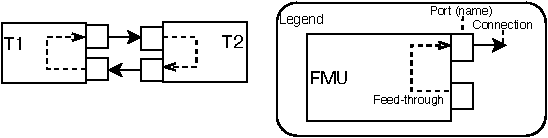
\includegraphics{images/fmu_cycle.pdf}
    \caption{Co-simulation scenario with cycle}
    \label{fig:fmu_cycle}
\end{figure}

\begin{definition}[Algebraic loops] 
The set of interconnected variables in an algebraic loop is defined as: $\LoopVariables = \{v | v \in V : Path(v,v)\}$ \\
An algebraic loop is defined as the set $\{p_1, p_2 | p_1, p_2 \in \LoopVariables: Path(p_1, p_2) \land Path(p_2, p_1)\}$\todo{Look at this - can it be specified better?}\\
Path is defined as the transitive closure of the set of relations: $\bigcup_{c \in \fmus} \set{\feedthrough{c}} \cup \coupling$\\
The algebraic dependency will lead to the following difference between performing to following :
\todo{Claudio check this definition and add a formalization of the challenge introduced}
\end{definition}

\begin{definition}[Challenge of Algebraic loops]\label{def:challenge}
The algebraic dependency will lead to the following difference between performing to following :
\todo{Claudio check the other definitions and add a formalization of the challenge introduced}
\end{definition}

As described by definition \ref{def:challenge} the algebraic loops introduce certain challenges in the system. This means that algebraic loops needs to be handled using fixed point iterations\cite{Gomes2018}. It is a technique to repeatedly perform the steps of a sub-list of the co-simulation step. The number of repetitions the operations should be be performed depends on the characteristics of the scenario. The operations should be performed until the system converge. 
An example of applying a fixed point iteration can be seen in Figure \ref{def:fixedpoint} where a system containing an algebraic loop has to be initialized using fixed point iteration.

\begin{figure}[H]
    \centering
    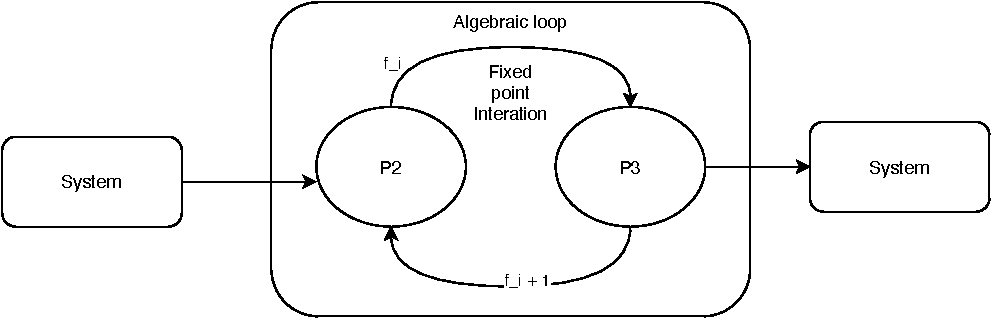
\includegraphics[width=0.8\textwidth]{images/fixedpoint.pdf}
    \caption{Fixed point iteration in a co-simulation scenario}
    \label{fig:fixedpont}
\end{figure}

The initialization of the system requires application of fixed point iteration as defined by definition \ref{def:fixedpoint}.
\begin{definition}[Fixed point iteration of an Initialization procedure]\label{def:fixedpoint}
Given an Initialization procedure $\sequence{\initcall_i}_{i \in \setnat}$ of a co-simulation $\tuple{\fmus, \coupling}$ where $\LoopVariables \neq \emptyset$.\\
Fixed point iteration should be used by 
$\forall v \in \LoopVariables $

\end{definition}

However a fixed point iteration technique is not guaranteed to convergence if the system is unstable. This means that an upper bound of the number of repetitions needs to be established to ensure termination. In case of a non-converging algebraic loop the simulation should be stopped since the result of the co-simulation scenario wouldn't be trustworthy. The criteria of a valid co-simulation scenario is is specified in definition \ref{def:convergence}.

\begin{definition}[Convergence of Fixed point iteration]\label{def:convergence}
A fixed point iteration is converging if a finite number of iterations will make the difference of the output-value of the same operation between two following iterations within a certain threshold.\\
$Convergence = \exists n \in \setnat: \forall p \in \LoopVariables \implies |f(p, n + 1) - f(p, n)| \leq T$\\
$f$ is the operation performed on a loop-variable p of a given iteration n.
\end{definition}


\subsection{INTO-CPS Maestro 2}\todo{We can have some more in this section - potentially half a page - Ask Casper if he can do it?}
INTO-CPS Maestro 2\footnote{currently in alpha \url{https://github.com/INTO-CPS-Association/maestro/tree/2.0.0-alpha}}\cite{thule_maestro2_2019} is an FMI-based co-simulation framework set to supersede Maestro\cite{Maestro}. The philosophy of the framework is to apply plugins to generate co-simulation specifications expressed in the domain specific language called Maestro Base Language (MaBL). Such specifications are then interpreted and executed resolving in the execution of a co-simulation.
